\section{形状計測試験(大野・奥山)}
\label{chap:shapemeasurement}

CubeSatはE-SSODと呼ばれるポッド内に収納された状態でロケットに搭載される.そのため,E-SSODに収まり,軌道上で問題なくE-SSODから放出されるために,CubeSatの形状には制約がある.本衛星の形状に関する要求は,インターフェース管理文書(以後ICDと記載)に定義されている.
ICDに記載されている形状に関する要求には以下のものがある.
\begin{enumerate}
	\item 外形寸法に関する要求
	\item レールに関する要求
	\item エンベロープに関する要求
	\item 質量特性に関する要求
	\item セパレーションスプリング/ディプロイメントスイッチ
	\item 強度要求
	\item アクセス窓
\end{enumerate}

これらの要求に関する試験結果についてはOrigamiSat-1検査成績書(OP-S1-0009)に記載されている.本章では,これらの要求の詳細と,要求を満たしているか確認するために行った試験について説明する.

\subsection{外形寸法に関する要求}

本衛星は3UのCubeSatであり,ICDにおいて寸法は以下のように規定されている

\begin{enumerate}
	\item 縦横ともに100$\pm$0.1 mmの幅とすること
	\item 高さは340.5 $\pm$0.3 mmとすること
\end{enumerate}

この要求が満たされているか確認するために,まず三次元測定機を用いた測定を行なった.

\subsubsection{三次元測定機を用いた測定}

東工大の工場内には図\ref{fig:3dmeasurementmachine}に示すような三次元測定機がある.三次元測定機とは,3次元で物体の各点の座標を測定することができる装置である.

\begin{figure}[h]
	\begin{center}
		
		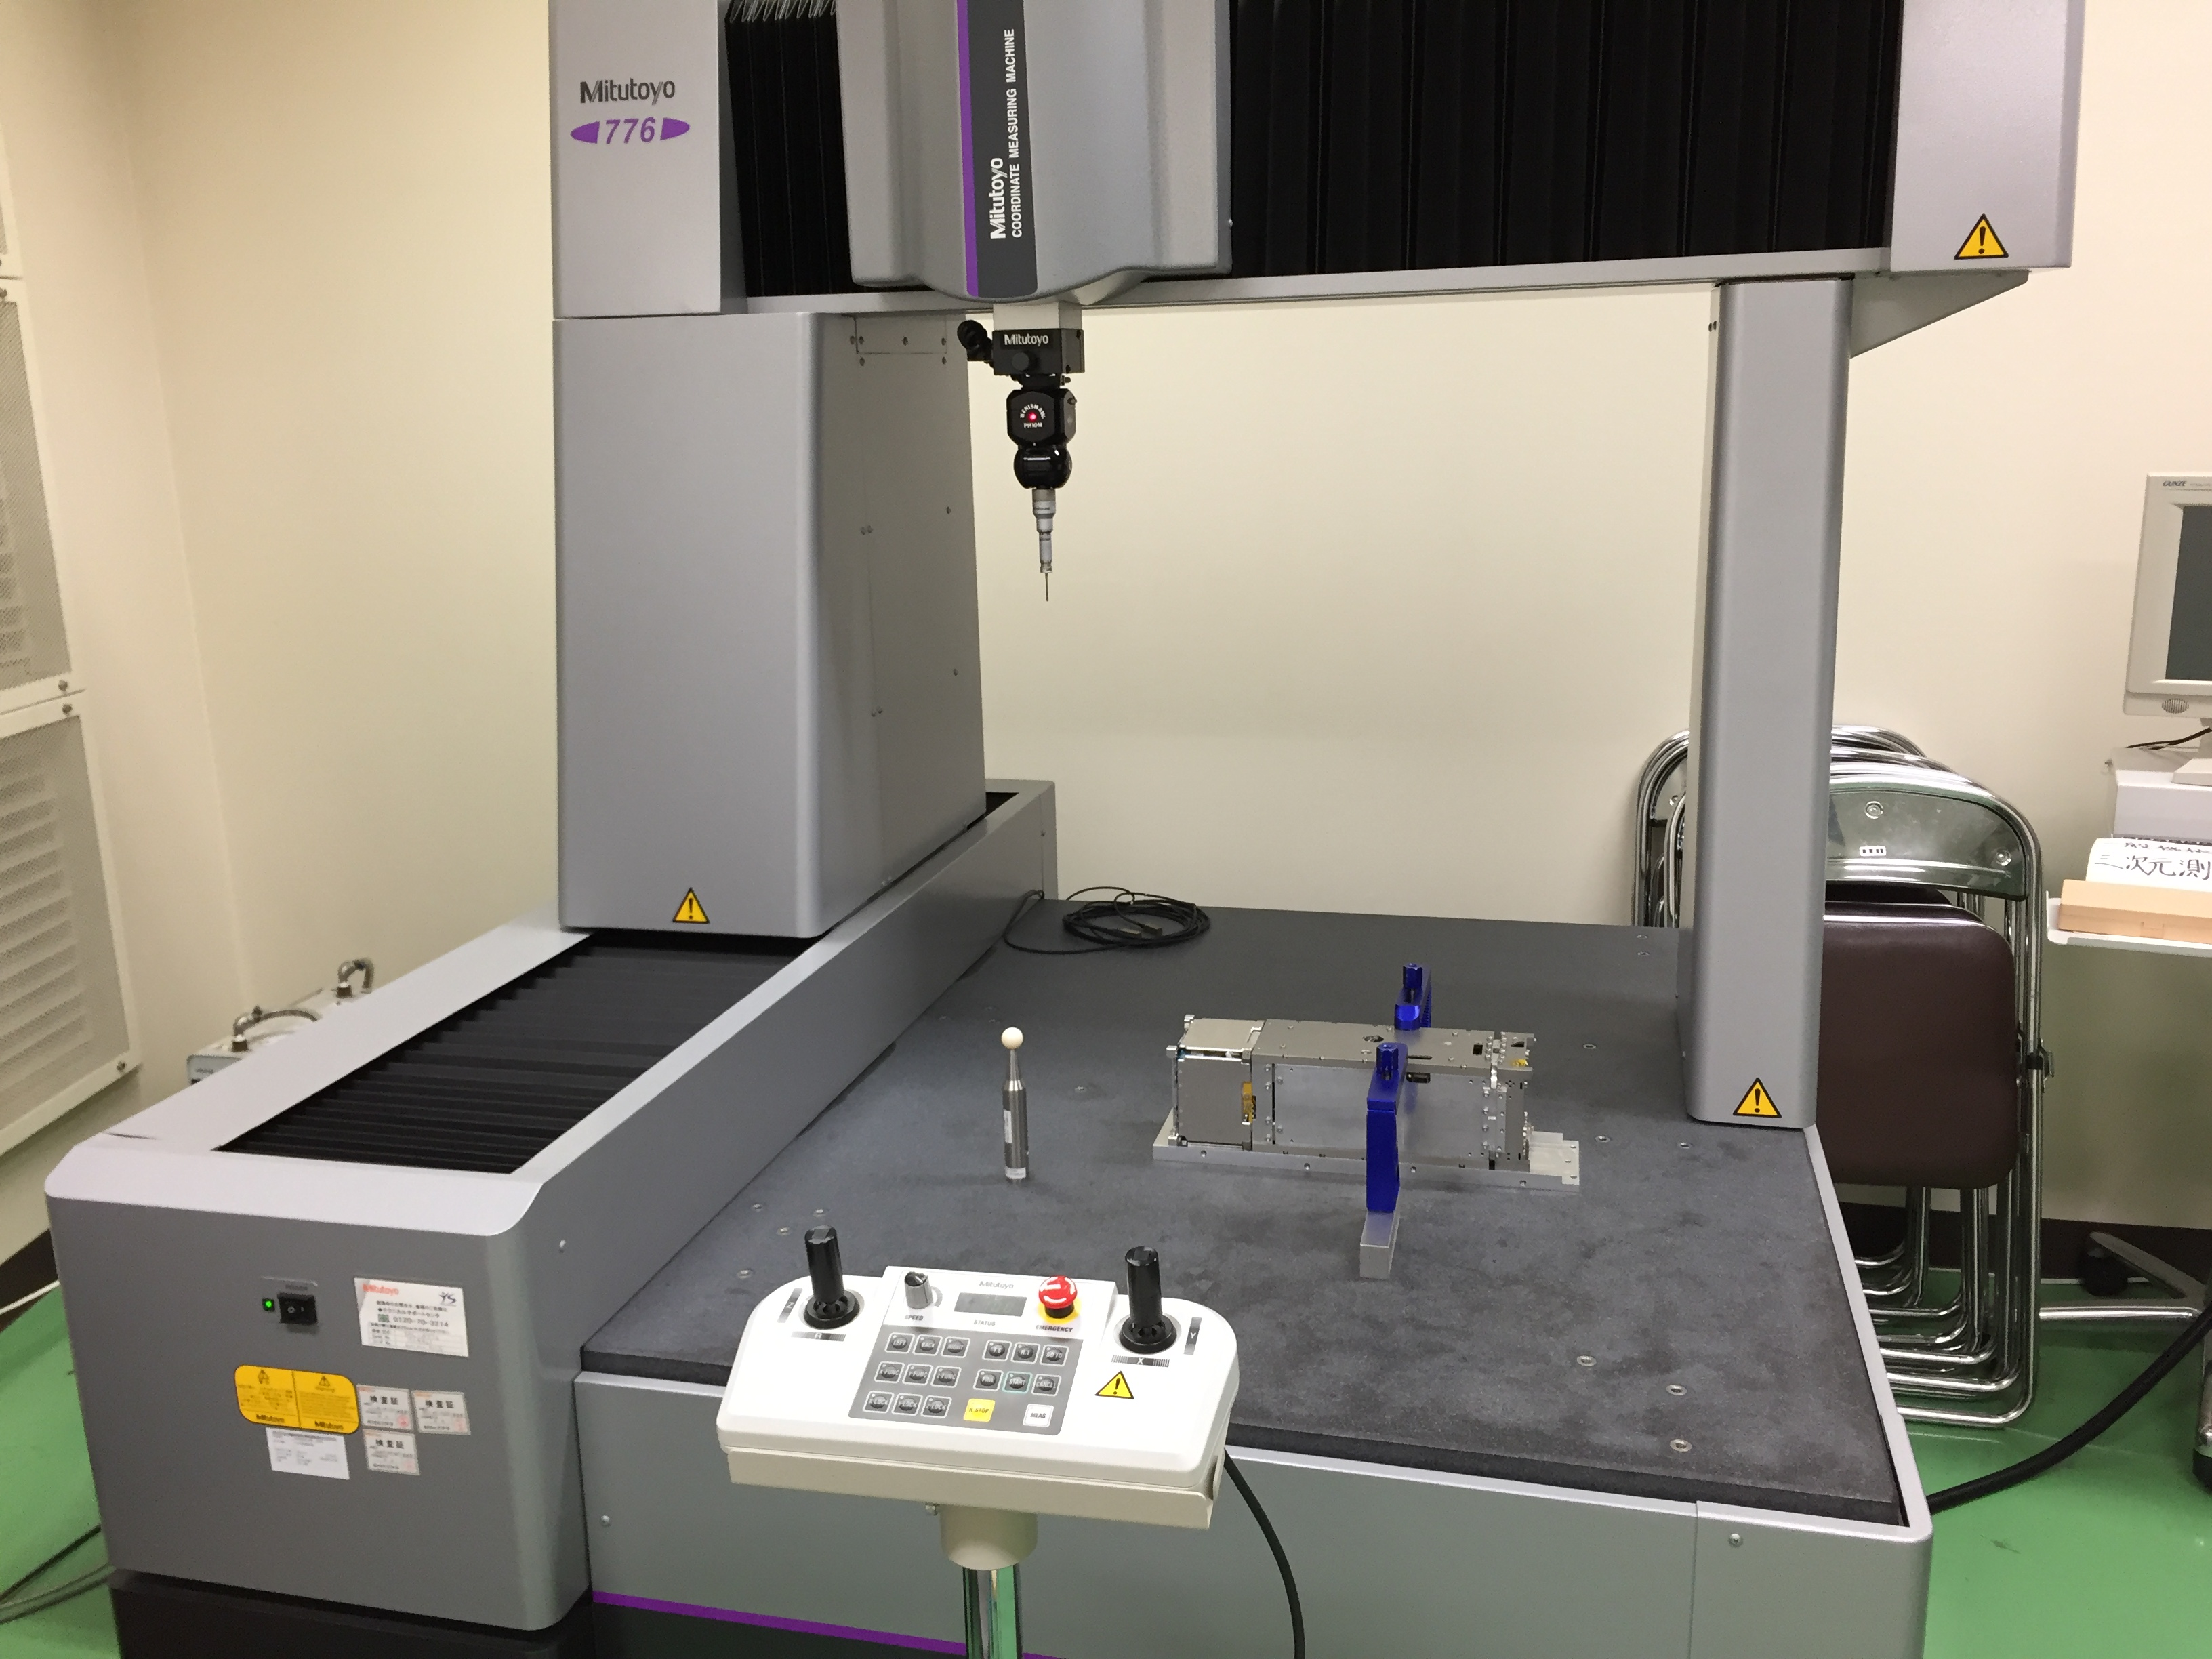
\includegraphics[width=0.6\linewidth]{04/fig/3dmeasurementmashine.JPG}
		\caption{3次元測定機}
		\label{fig:3dmeasurementmachine}
		
	\end{center}
\end{figure}

三次元測定機は,工場特殊セルフ利用にあたり,通常の工場利用の際に受ける講習だけではなく,三次元測定機の利用講習を受ける必要がある.三次元測定機の利用講習は,業務依頼書に講習希望の旨を記入しメールで提出する.講習を受けたのち,工場に利用予約のメールをし,予約が空いていれば教員立ち会いのもと使用することができる.工場特殊セルフ利用は通常の工場利用よりも時間単価が高く,利用には注意が必要である.

本衛星の測定には,衛星のレールに沿って座標軸を設定し,そのレールに対し対面のレールが100$\pm$0.1 mmの幅で収まっているか確認するという方法を用いた.測定結果を入力すると,正しい位置からの誤差を拡大して表示し,ずれている方向をわかりやすく示すExcelシートを作成した.結果は以下の図\ref{fig:3dmeasurementresult}のように表示される.

\begin{figure}[h]
	\begin{center}
		
		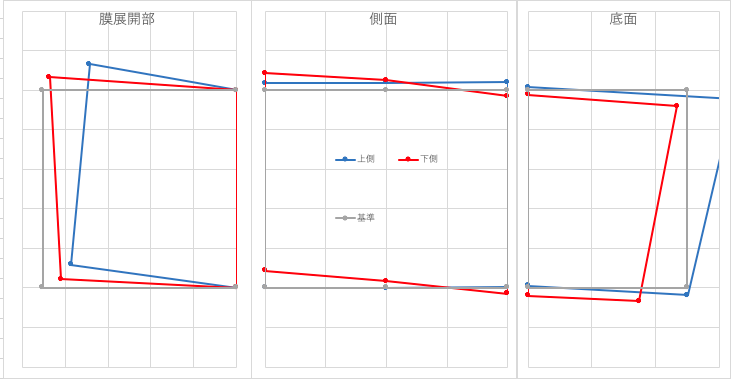
\includegraphics[width=0.8\linewidth]{04/fig/3dmeasurementresult.png}
		\caption{3次元測定結果図示}
		\label{fig:3dmeasurementresult}
		
	\end{center}
\end{figure}

測定結果が要求を満たしていなかった場合には,一旦ネジを緩め再度精度出しを行った.精度出しをやり直す際には,Excelで図示した結果をもとにはみ出している箇所と治具のレール部の間にシムテープを挟み誤差の修正を行った.シムテープを挟み込むことで誤差を調整することはできるが,EM,FMともに完全に要求を満たすことはできなかった.

三次元測定はJAXAやIHI Aerospace(以後IAと記載)から指定された測定手法ではなく,外形寸法の要求を満たしているか確認するために,東工大側で選択した確認方法である.開発スケジュールに遅れが出ていたこともあり,要求を満たしているか確認する方法を変更することにした.

\subsubsection{フィットチェックとノギスによる確認}

フィットチェックとはE-SSODに衛星が収まるかどうかを,フィットチェック用PODに衛星を収納することで確認する作業である.E-SSODのレール幅は100.5$\pm$0.2 mmであるが,フィットチェック用PODのレール幅は100.2$\pm$0.1 mmとなっており,フィットチェック用PODに引っかかりなく収納されればE-SSODに問題なく収めることができる.フィットチェックの様子を以下の図\ref{fig:fitcheck}に示す.

\begin{figure}[h]
	\begin{center}
		
		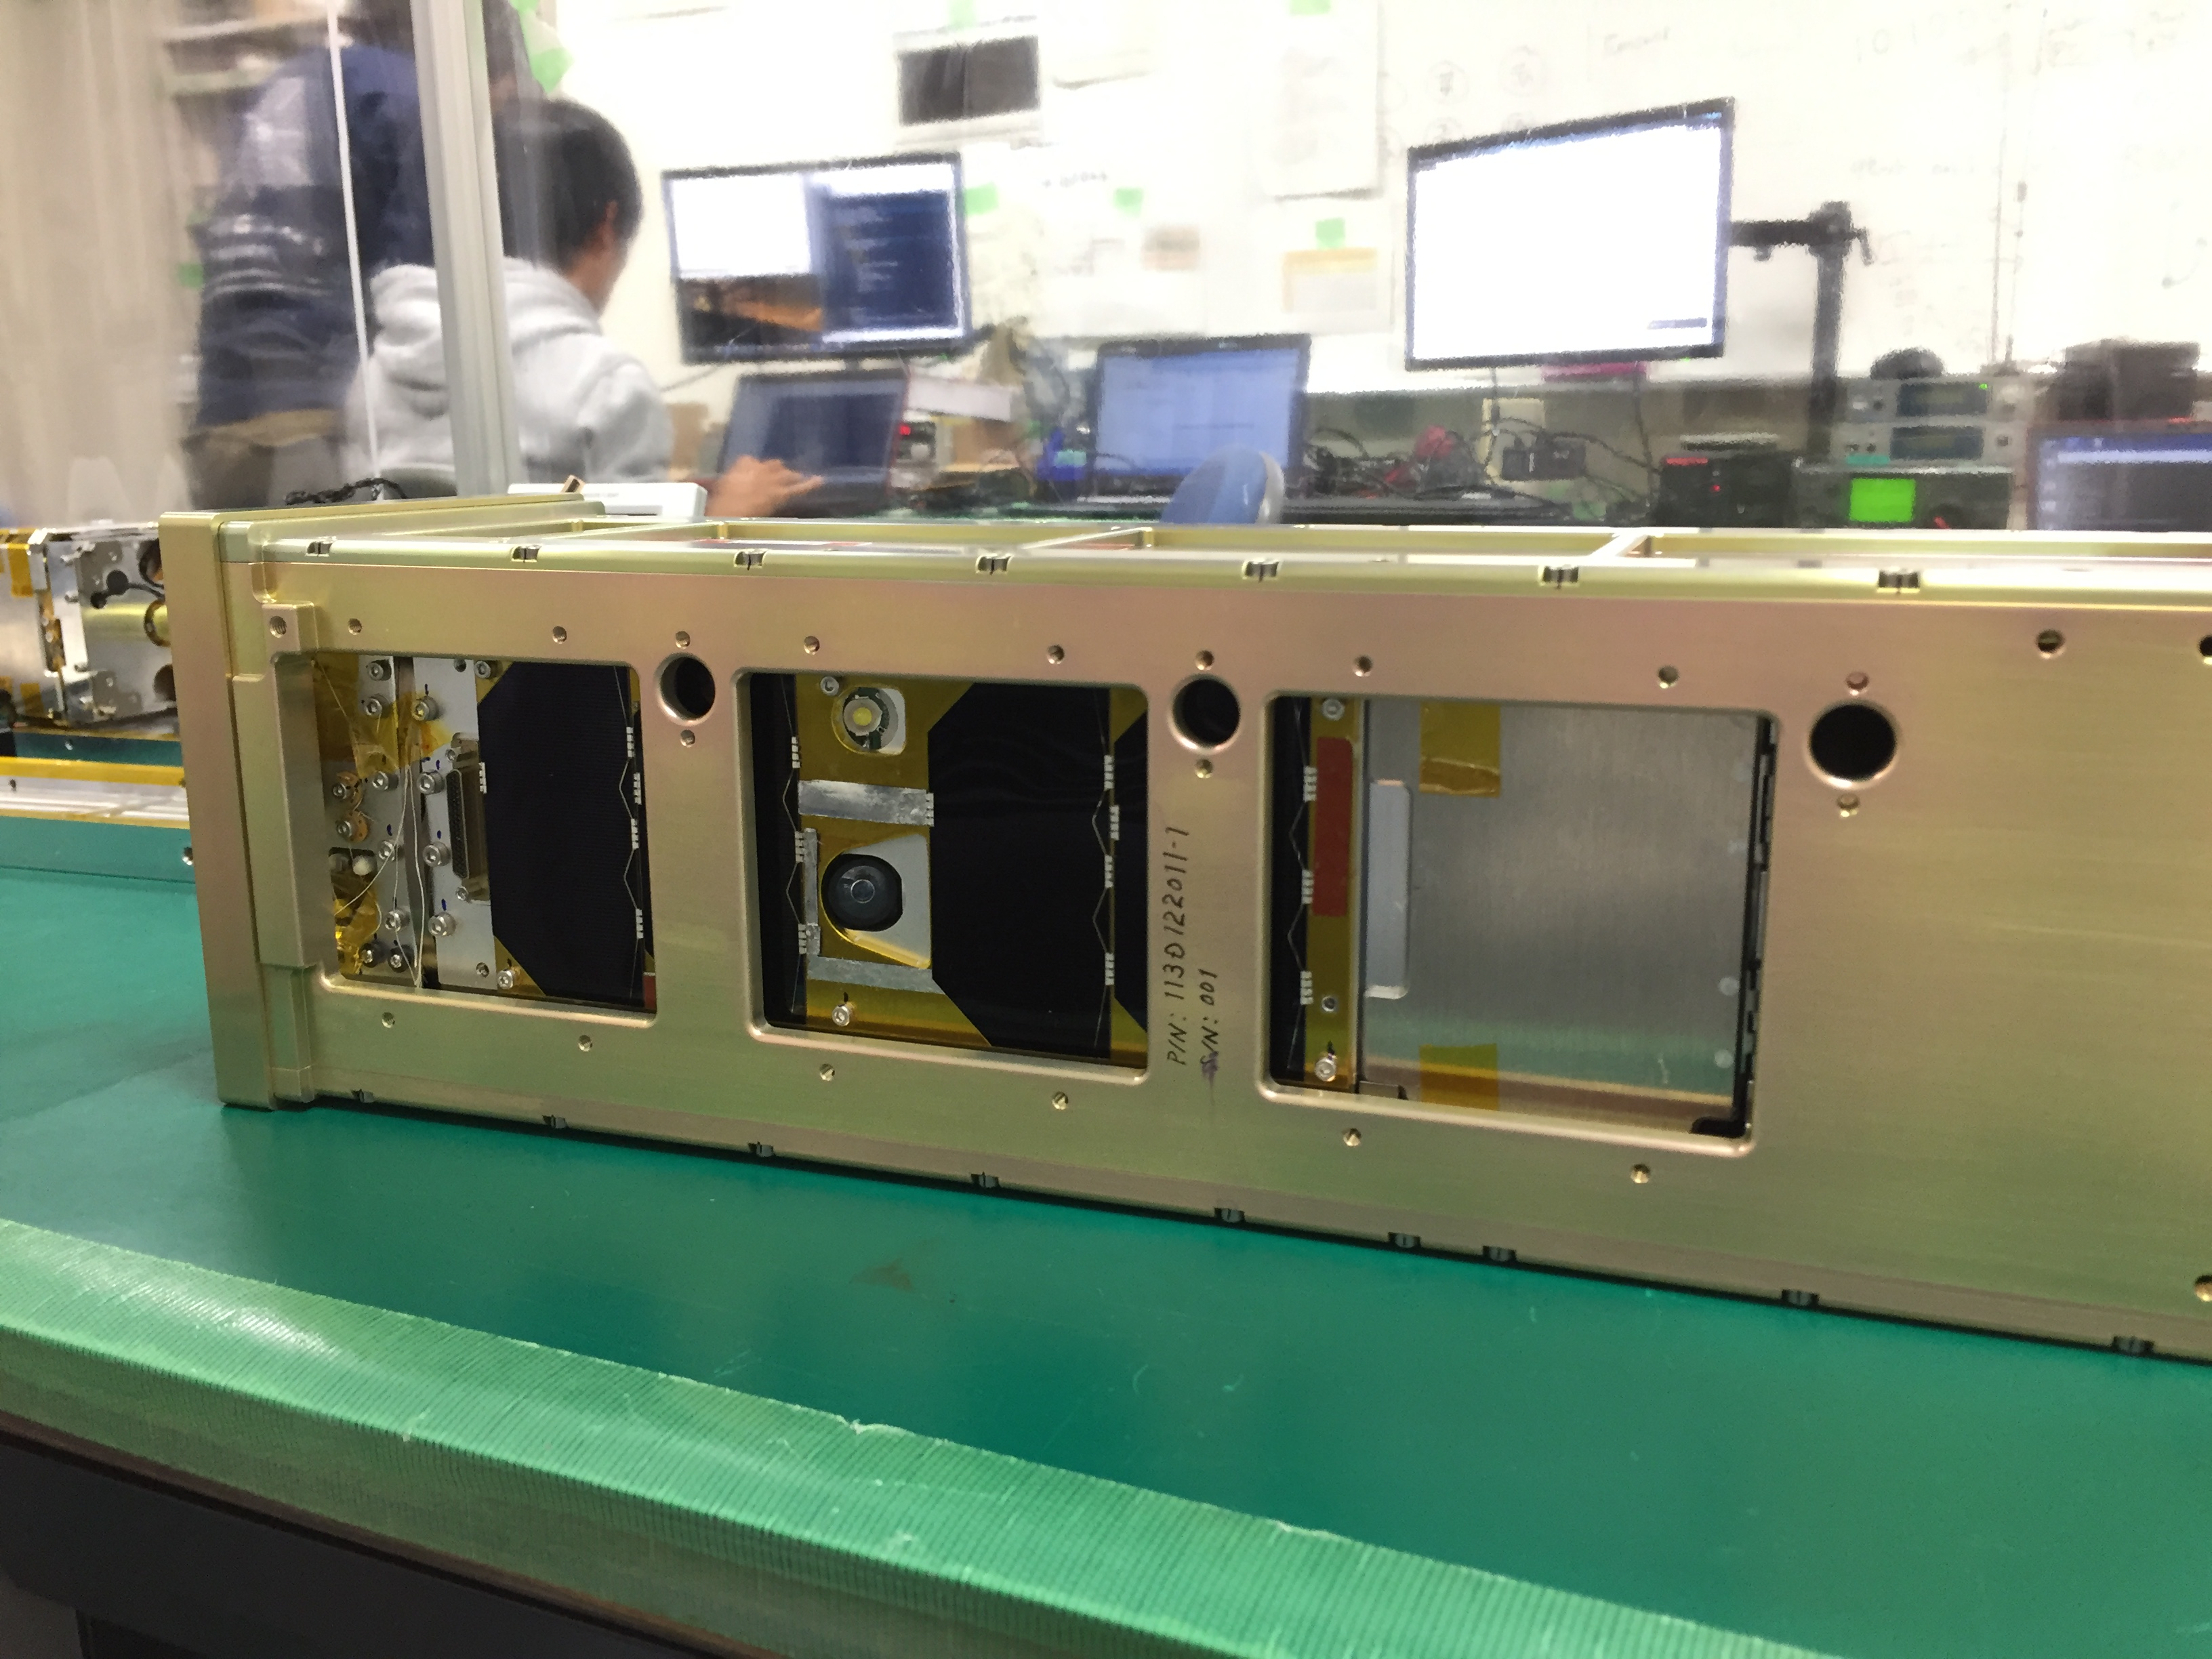
\includegraphics[width=0.6\linewidth]{04/fig/fitcheck.JPG}
		\caption{フィットチェックの様子}
		\label{fig:fitcheck}
		
	\end{center}
\end{figure}

本衛星の外形寸法の要求確認は,フィットチェックでPODに問題なく収まることを確認したのちに,ノギスで各部のレール幅を測るという方法で行うこととした.フィットチェックは引っかかりなく収まることを確認するために,動画で記録している.

この検査方法では精度出しをやり直すことなく1回でフィットチェック用ポッドに収まり,ノギスでの測定でも問題は生じなかった.より詳細な検査結果は検査成績書を参照のこと.

\subsection{レールに関する要求}

レールはE-SSODと衛星が接する部分であり,打ち上げ時に衛星を支え,放出時にはガイドとなるため,とても重要度が高くICDでは8つの項目が規定されている.その中で本衛星にとって問題となった要求が以下の2つである.

\begin{enumerate}
	\item レールの表面はRa1.6 $\mu$m以下とすること
	\item 各レールの$\pm$Zを除く側面について,E-SSODのガイドレールと少なくとも75\%以上接触面を持つこと
\end{enumerate}

レール表面粗さについてはFM側面パネル発注時に,図面上で表面粗さの指定を間違えていたため要求が満たされておらず,別途表面粗さ計測試験を行った.詳細は第\ref{chap:surfaceroughness}章を参照のこと.またレール長さについては,設計上長さの規定を満たしていなかった.本衛星には膜展開部や,側面パネルと底面パネルの間などレールではない部分が多くある.この長さの分は設計時に考慮できていたが,側面パネル固定のためのネジ穴の座繰り分を計算に入れておらずレール長さが規定より短くなってしまった.そのため,規定より短い長さのレールでも問題なくE-SSODから放出できるか確かめるために放出試験を行った.詳細は第\ref{chap:ejectiontest}章を参照のこと.その他の要求についての検査は検査成績書に記載されている.

\subsection{エンベロープに関する要求}

エンベロープに関する要求とは,衛星のレール面より内部の突起物に関する要求である.突起物のレール面からの距離,突起部の長さが規定されている.また,展開構造についても誤展開した際の安全性に関して要求がなされている.

本衛星は突起物に関しては設計上問題はないが,展開構造に関しては展開アンテナの厚さが要求を満たしておらず,冗長系のテグスを巻くことで安全性を担保している.詳しい検査結果は検査成績書に記載されている

\subsection{質量特性に関する要求}

質量特性に対する要求は以下の2つであった.

\begin{enumerate}
	\item 質量が1Uあたり0.13kg以上,1.5kg以下であること
	\item 質量中心が4本のレールで構成される直方体の幾何中心を中心とする半径20mmの球体内に位置すること
\end{enumerate}

質量については,本衛星は3Uであるため質量が0.39kg以上,4.5kg以下であれば良い.実際の質量はCADで確認したのちに,組み立て前にコンポーネントごとに質量計測し,組み立て後に衛星全体の質量を測定した.

質量中心はCAD上で計算している.

\subsection{セパレーションスプリング/ディプロイメントスイッチに関する要求}

衛星がE-SSODから放出されたことを確認する衛星側のスイッチに関する要求である.本衛星は設計段階からこの要求を満たしている.放出検知スイッチの電気的な要求の確認方法については組立手順書を参照のこと.

\subsection{強度要求}
衛星が地上,試験,運搬,打ち上げ,運用の過程において破損や永久変形しないことを求める要求である.強度要求は衝撃試験,振動試験で確認を行った.

\subsection{アクセス窓}
アクセス窓はE-SSODに収納後に衛星にアクセスする必要がある際のアクセスポート設置位置に関する要求である.E-SSODは引き渡し時に蓋を閉めたのちに開けることはないため,ソフトの書き換え,フライトピンなど衛星にアクセスする必要に備えてアクセスポートを設置しておく.

本衛星はバス部のソフト書き換え用にD-subコネクタを備えており,E-SSODのアクセス窓からアクセスが可能である.また,このアクセスポートは振動試験の際にも以下の図\ref{fig:accessport}のように,衛星内部の機器と接続するために必要となる.振動試験の際に衛星の収納方向を入れ替えたが,入れ替えた後もD-subコネクタはアクセス窓からアクセス可能であった.なお,MDCボックスに設けられているmicroD-subのコネクタはMDCソフト書き込み用のものである.組立後にMDCにアクセスできなくなるため設けられたもので,アクセス窓に関する要求とは無関係のものである.

\begin{figure}[h]
	\begin{center}
		
		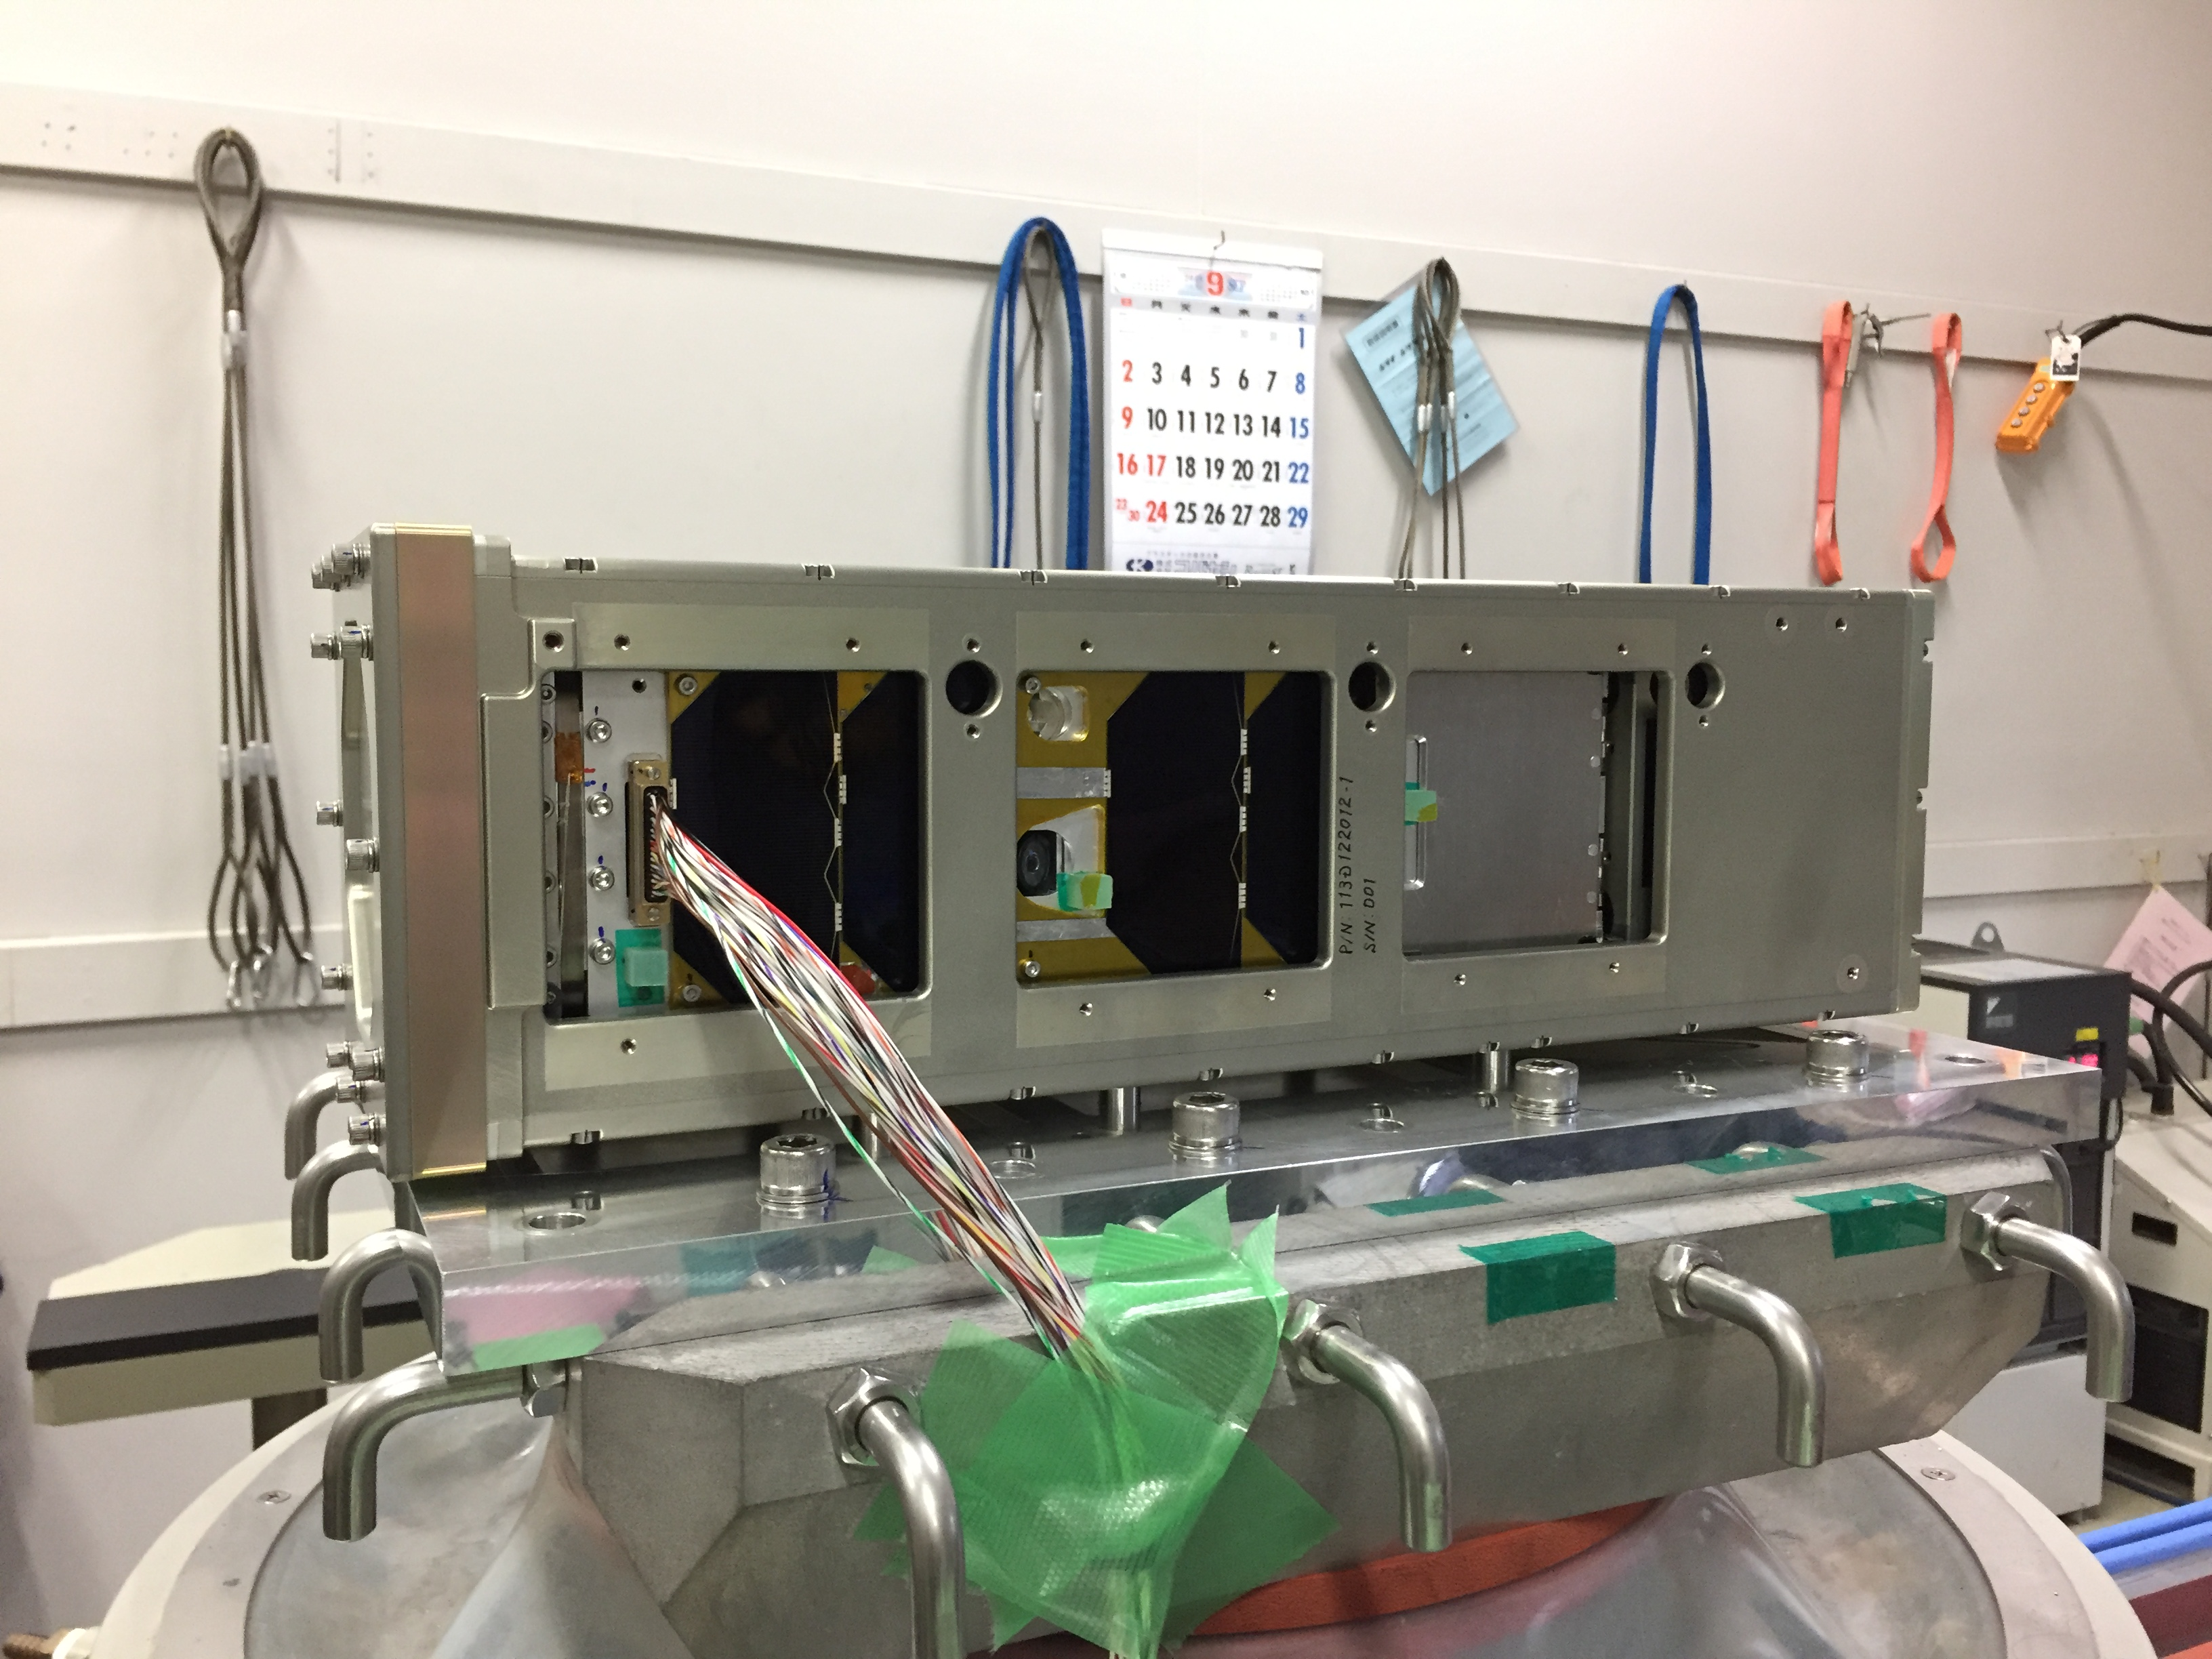
\includegraphics[width=0.6\linewidth]{04/fig/accessport.JPG}
		\caption{振動試験時のアクセスポート利用}
		\label{fig:accessport}
		
	\end{center}
\end{figure}